\section{Rotor do sterowania antenami w płaszczyźnie azymutu i elewacji}

Konstrukcja rotora składa się z dwóch stalowych skrzynek osłaniających silniki. W skrzynkach zostały wykonane otwory na poprowadzenie przewodów do zasilania i sterowania.

Aby uzyskać dużą precyzję i wytrzymały na warunki zewnętrzne system pomimo małych gabarytów, potrzebne było duże przełożenie dla silników. Po doborze przekładni pełen obrót w płaszczyźnie azymutu zajmuje 124 sekundy, a w płaszczyźnie elewacji 64 sekundy. Wolny czas obrotu zwykle w rotorach antenowych nie przeszkadza, ponieważ zwykle nie namierza się szybko poruszających się źródeł sygnału. 

Śledzimy pozycję rotora przy pomocy zestawu czujników: 
\begin{itemize}
 \item enkoderów optycznych przed przekładnią (co znacznie poprawia ich rozdzielczość na pełen obrót, ale wprowadza trochę błędu ze względu na luzy w przekładniach)
 \item zamontowanego do obracającej się osi układu zawierającego kompas magnetyczny, i żyroskopy i akcelerometry w trzech osiach, który służy do kalibracji układu i wykrycia konieczności wprowadzania ewentualnej korekty do obliczeń orientacji (jeśli rotor stoi np. na pochyłym podłożu).
\end{itemize}

\begin{figure}[!htbp]
 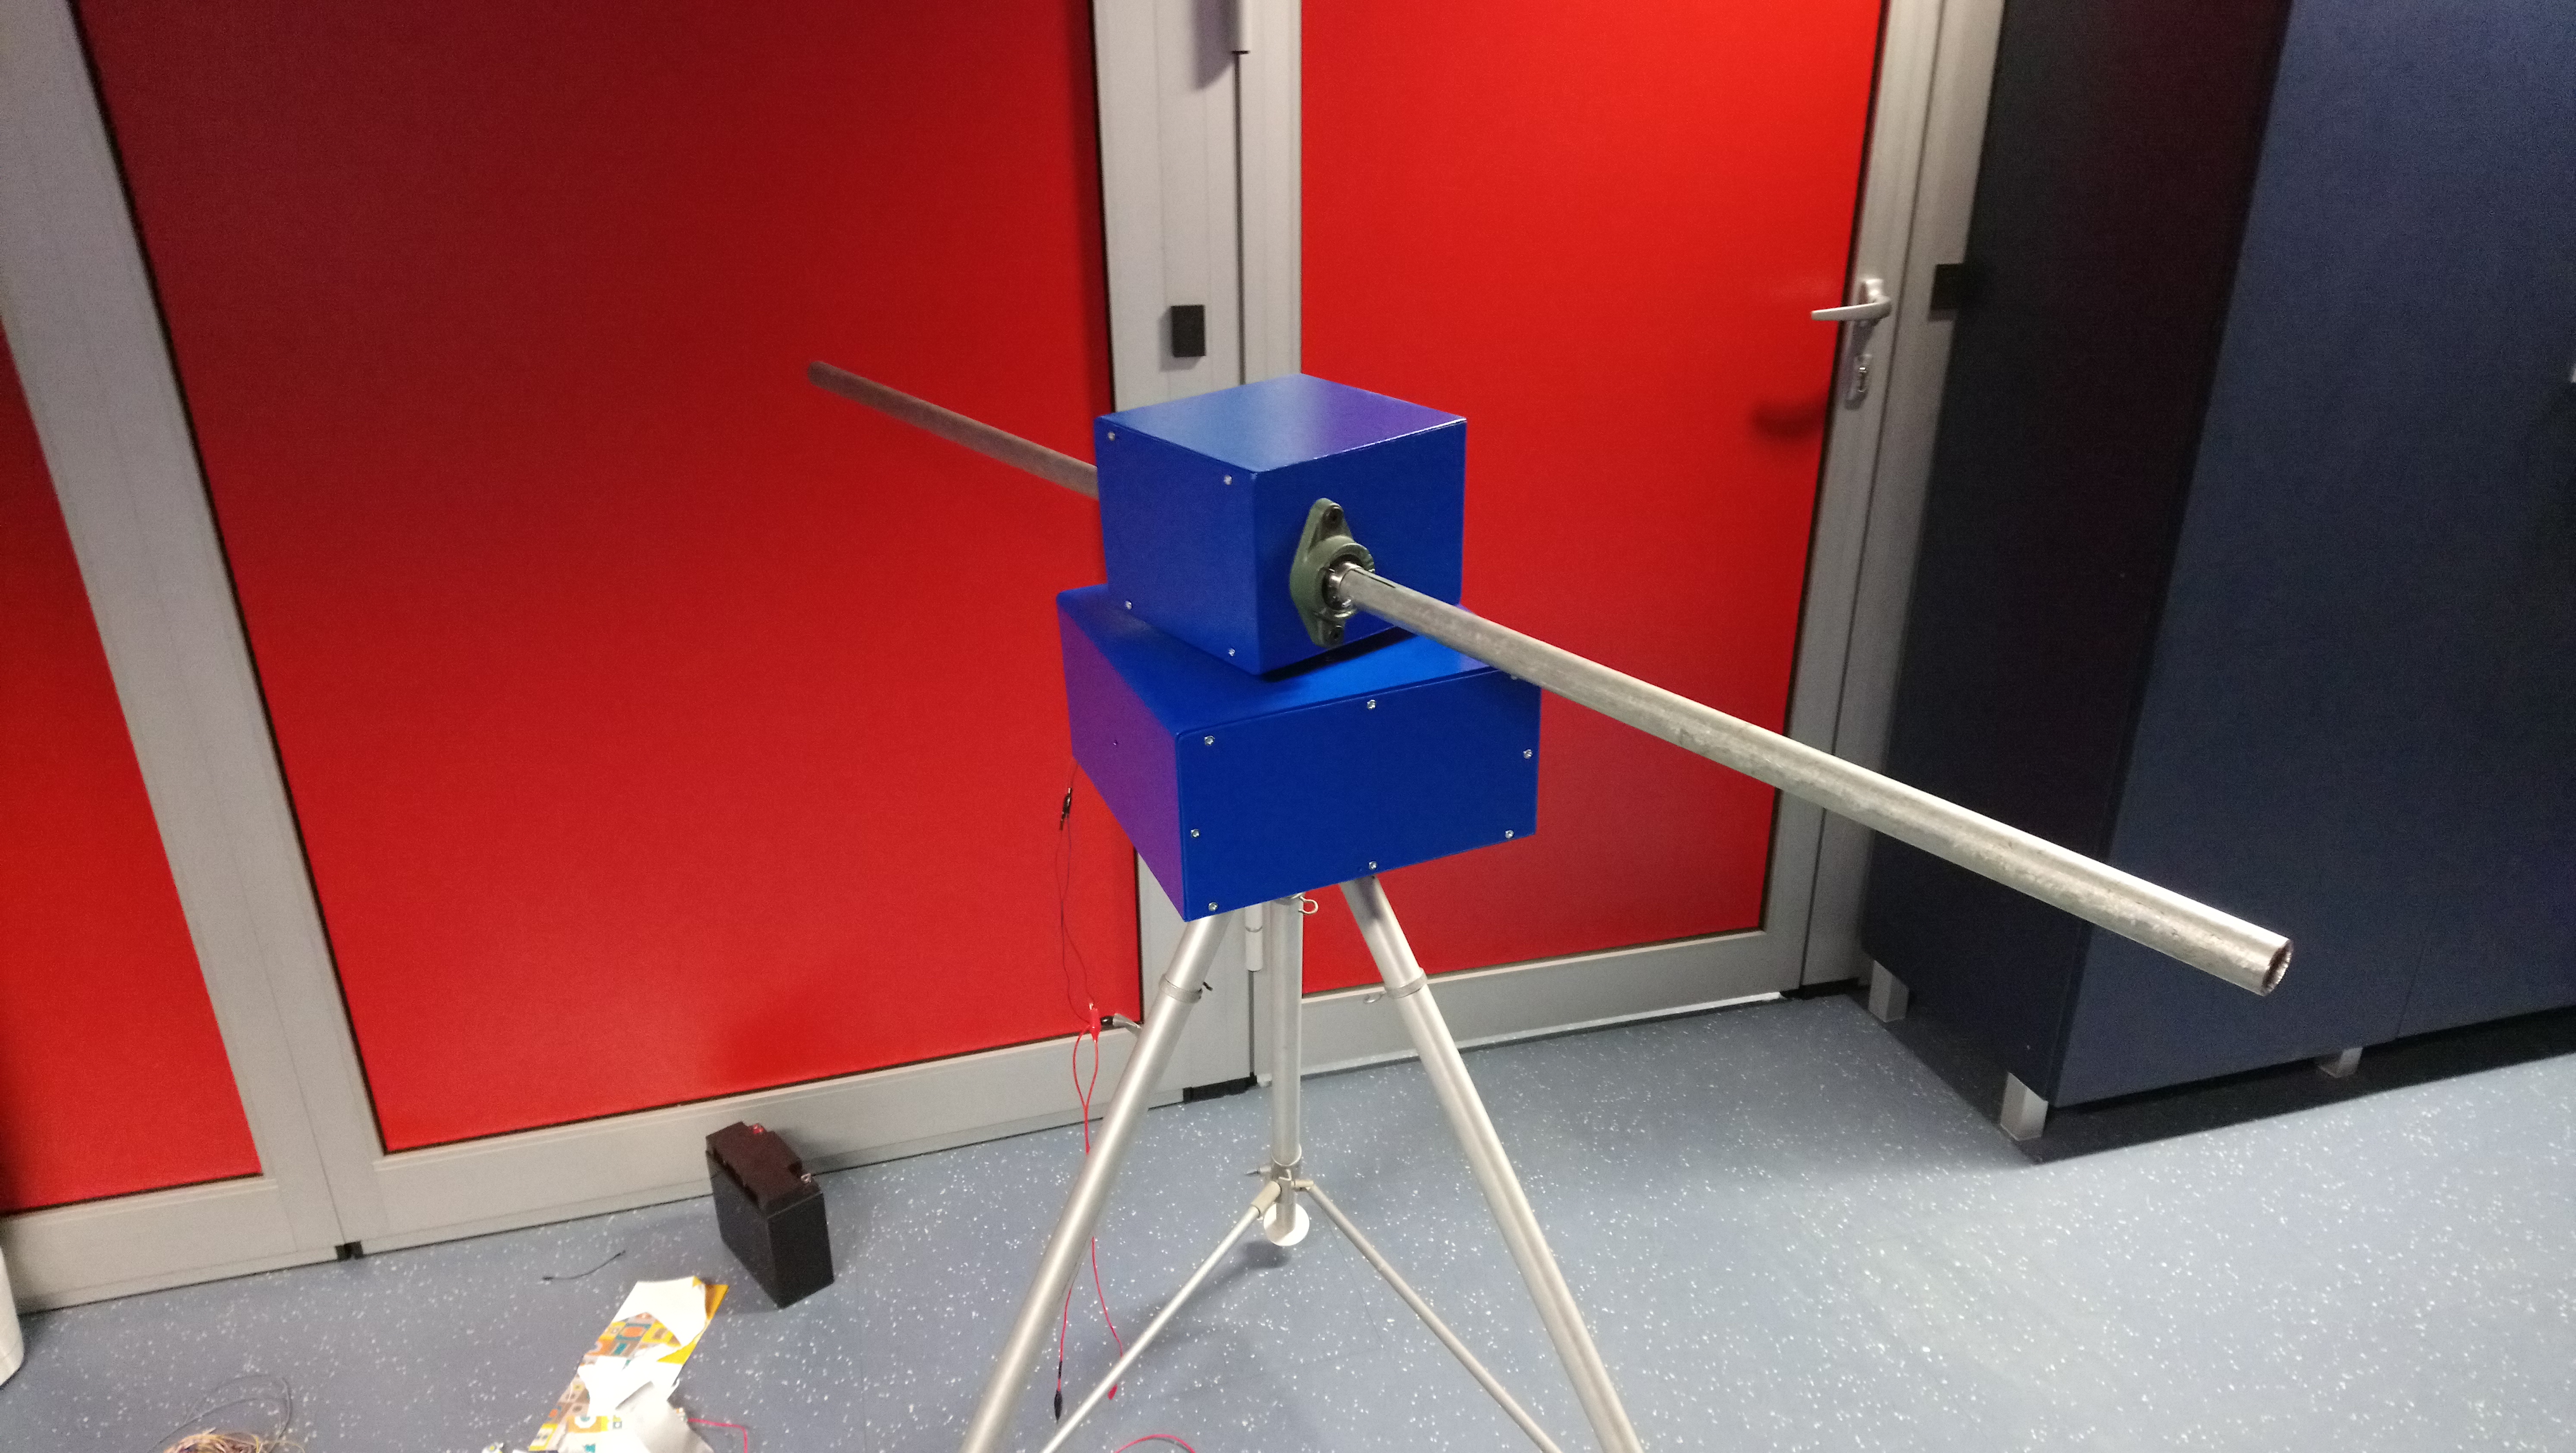
\includegraphics[width=0.8\textwidth]{rotor}
 \centering
 \caption{Konstrukcja rotora zamontowana na statywie}
\end{figure}

Cała stacja waży około 12 kilogramów. Rotor ma miejsce na przykręcane rury do mocowania anten. Przewidujemy nie więcej niż 2 anteny jednocześnie o łącznej wadze do 8 kilogramów.

Niestety tak jak w większości rotorów (poza zaawansowanymi sztuczkami), ze względu na kabel nie możemy obracać rotora w tym samym kierunku bez ustanku. Maksymalny kąt obrotu zależy od poprowadzenia przewodu zarówno do anteny jak i zasilających w rotorze. Do zasilania daliśmy zapas kabla na około 2 pełne obroty. Pilnowanie aby nie przekroczyć maksymalnego obrotu odbywa się programowo zapamiętując i wczytując względny obrót w pamięci trwałej. 

Rotor bardzo trudno obrócić bez włączonego zasilania ze względu na przekładnie. Jest to zamierzone, aby przy trudniejszych warunkach atmoseferycznych (przede wszystkim wietrze) rotor się nie obracał bez kontroli.
